\documentclass{standalone}
\usepackage{tikz}
\usetikzlibrary{patterns, positioning}

\begin{document}
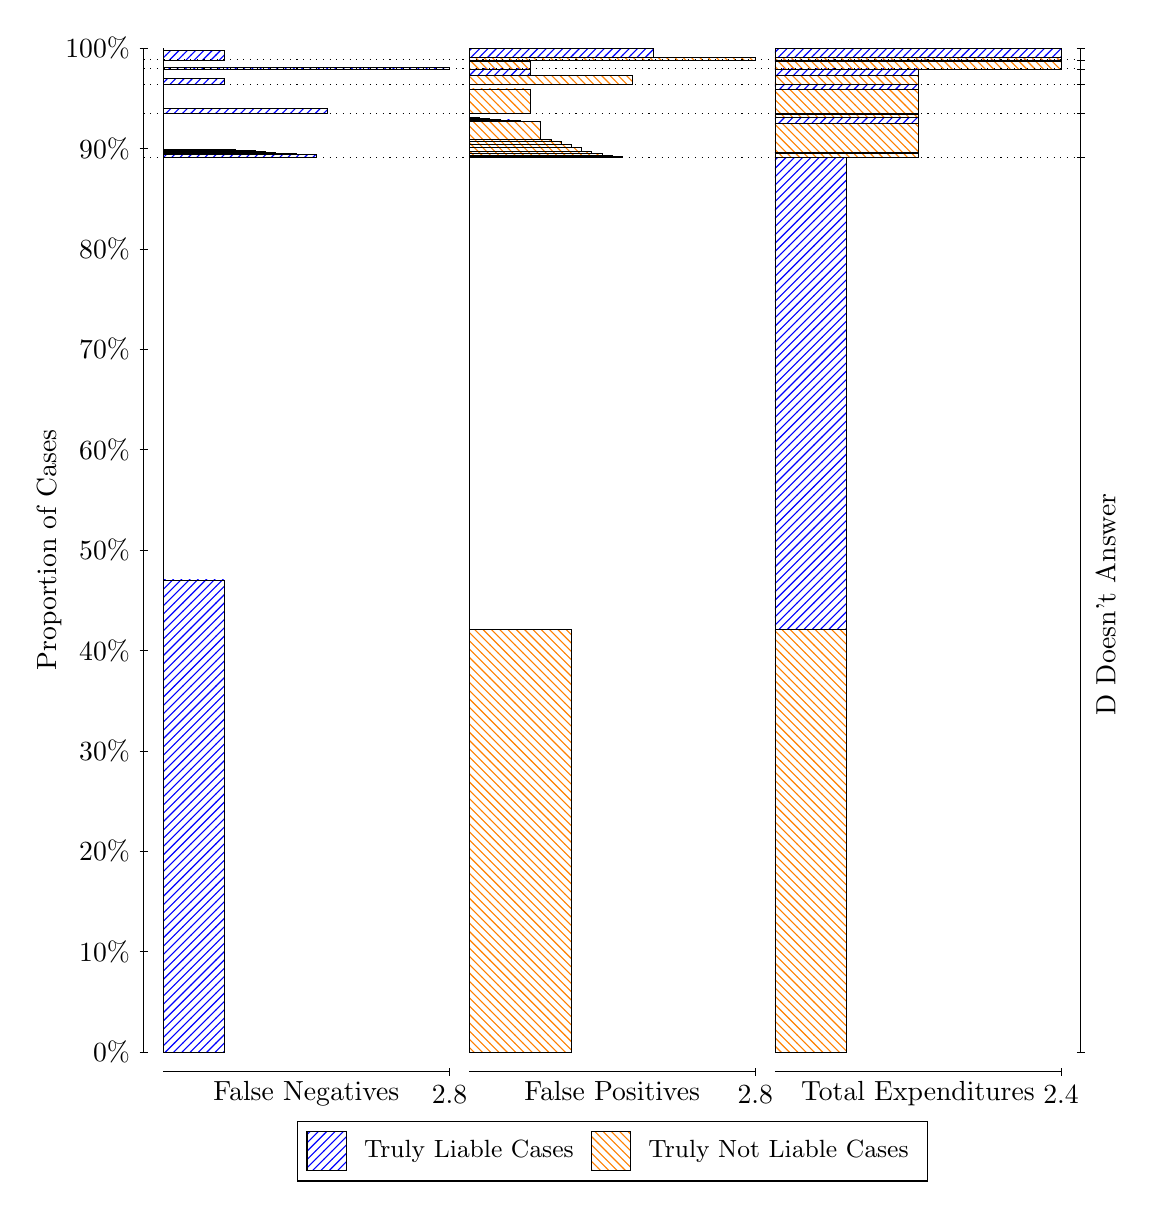
\begin{tikzpicture}
\draw[black, very thin] (1.5,1.75) -- (1.5,14.5);
\node[rotate=90, anchor=center] at (0.3, 8.125) {Proportion of Cases};
\draw[black, very thin] (1.45,1.75) -- (1.55,1.75);
\node[anchor=east] at (1.45, 1.75) {0\%};
\draw[black, very thin] (1.45,3.025) -- (1.55,3.025);
\node[anchor=east] at (1.45, 3.025) {10\%};
\draw[black, very thin] (1.45,4.3) -- (1.55,4.3);
\node[anchor=east] at (1.45, 4.3) {20\%};
\draw[black, very thin] (1.45,5.575) -- (1.55,5.575);
\node[anchor=east] at (1.45, 5.575) {30\%};
\draw[black, very thin] (1.45,6.85) -- (1.55,6.85);
\node[anchor=east] at (1.45, 6.85) {40\%};
\draw[black, very thin] (1.45,8.125) -- (1.55,8.125);
\node[anchor=east] at (1.45, 8.125) {50\%};
\draw[black, very thin] (1.45,9.4) -- (1.55,9.4);
\node[anchor=east] at (1.45, 9.4) {60\%};
\draw[black, very thin] (1.45,10.675) -- (1.55,10.675);
\node[anchor=east] at (1.45, 10.675) {70\%};
\draw[black, very thin] (1.45,11.95) -- (1.55,11.95);
\node[anchor=east] at (1.45, 11.95) {80\%};
\draw[black, very thin] (1.45,13.225) -- (1.55,13.225);
\node[anchor=east] at (1.45, 13.225) {90\%};
\draw[black, very thin] (1.45,14.5) -- (1.55,14.5);
\node[anchor=east] at (1.45, 14.5) {100\%};

\draw[black, very thin] (13.4,1.75) -- (13.4,14.5);
\draw[black, very thin] (13.35,1.75) -- (13.45,1.75);
\node[anchor=west] at (13.35, 1.75) {};
\draw[black, very thin] (13.35,13.113) -- (13.45,13.113);
\node[anchor=west] at (13.35, 13.113) {};
\draw[black, very thin] (13.35,13.67) -- (13.45,13.67);
\node[anchor=west] at (13.35, 13.67) {};
\draw[black, very thin] (13.35,14.04) -- (13.45,14.04);
\node[anchor=west] at (13.35, 14.04) {};
\draw[black, very thin] (13.35,14.235) -- (13.45,14.235);
\node[anchor=west] at (13.35, 14.235) {};
\draw[black, very thin] (13.35,14.349) -- (13.45,14.349);
\node[anchor=west] at (13.35, 14.349) {};
\draw[black, very thin] (13.35,14.5) -- (13.45,14.5);
\node[anchor=west] at (13.35, 14.5) {};

\draw[black, very thin, pattern color=blue, pattern=north east lines] (1.75,1.75) rectangle (2.5286,7.7445);
\draw[black, very thin, pattern color=orange, pattern=north west lines] (1.75,7.7445) rectangle (1.75,13.113);
\draw[black, very thin, pattern color=blue, pattern=north east lines] (1.75,13.113) rectangle (3.6964,13.149);
\draw[black, very thin, pattern color=blue, pattern=north east lines] (1.75,13.149) rectangle (3.5667,13.153);
\draw[black, very thin, pattern color=blue, pattern=north east lines] (1.75,13.153) rectangle (3.4369,13.16);
\draw[black, very thin, pattern color=blue, pattern=north east lines] (1.75,13.16) rectangle (3.3071,13.166);
\draw[black, very thin, pattern color=blue, pattern=north east lines] (1.75,13.166) rectangle (3.1774,13.178);
\draw[black, very thin, pattern color=blue, pattern=north east lines] (1.75,13.178) rectangle (3.0476,13.186);
\draw[black, very thin, pattern color=blue, pattern=north east lines] (1.75,13.186) rectangle (2.9179,13.196);
\draw[black, very thin, pattern color=blue, pattern=north east lines] (1.75,13.196) rectangle (2.7881,13.2);
\draw[black, very thin, pattern color=blue, pattern=north east lines] (1.75,13.2) rectangle (2.6583,13.211);
\draw[black, very thin, pattern color=orange, pattern=north west lines] (1.75,13.211) rectangle (1.75,13.67);
\draw[black, very thin, pattern color=blue, pattern=north east lines] (1.75,13.67) rectangle (3.8262,13.729);
\draw[black, very thin, pattern color=orange, pattern=north west lines] (1.75,13.729) rectangle (1.75,14.04);
\draw[black, very thin, pattern color=blue, pattern=north east lines] (1.75,14.04) rectangle (2.5286,14.119);
\draw[black, very thin, pattern color=orange, pattern=north west lines] (1.75,14.119) rectangle (1.75,14.235);
\draw[black, very thin, pattern color=blue, pattern=north east lines] (1.75,14.235) rectangle (5.3833,14.257);
\draw[black, very thin, pattern color=orange, pattern=north west lines] (1.75,14.257) rectangle (1.75,14.349);
\draw[black, very thin, pattern color=blue, pattern=north east lines] (1.75,14.349) rectangle (2.5286,14.472);
\draw[black, very thin, pattern color=orange, pattern=north west lines] (1.75,14.472) rectangle (1.75,14.5);
\draw[black, very thin, pattern color=orange, pattern=north west lines] (5.6333,1.75) rectangle (6.931,7.1189);
\draw[black, very thin, pattern color=blue, pattern=north east lines] (5.6333,7.1189) rectangle (5.6333,13.113);
\draw[black, very thin, pattern color=orange, pattern=north west lines] (5.6333,13.113) rectangle (7.5798,13.123);
\draw[black, very thin, pattern color=orange, pattern=north west lines] (5.6333,13.123) rectangle (7.45,13.134);
\draw[black, very thin, pattern color=orange, pattern=north west lines] (5.6333,13.134) rectangle (7.3202,13.162);
\draw[black, very thin, pattern color=orange, pattern=north west lines] (5.6333,13.162) rectangle (7.1905,13.191);
\draw[black, very thin, pattern color=orange, pattern=north west lines] (5.6333,13.191) rectangle (7.0607,13.243);
\draw[black, very thin, pattern color=orange, pattern=north west lines] (5.6333,13.243) rectangle (6.931,13.278);
\draw[black, very thin, pattern color=orange, pattern=north west lines] (5.6333,13.278) rectangle (6.8012,13.314);
\draw[black, very thin, pattern color=orange, pattern=north west lines] (5.6333,13.314) rectangle (6.6714,13.339);
\draw[black, very thin, pattern color=orange, pattern=north west lines] (5.6333,13.339) rectangle (6.5417,13.572);
\draw[black, very thin, pattern color=blue, pattern=north east lines] (5.6333,13.572) rectangle (6.2821,13.584);
\draw[black, very thin, pattern color=blue, pattern=north east lines] (5.6333,13.584) rectangle (6.1524,13.588);
\draw[black, very thin, pattern color=blue, pattern=north east lines] (5.6333,13.588) rectangle (6.0226,13.597);
\draw[black, very thin, pattern color=blue, pattern=north east lines] (5.6333,13.597) rectangle (5.8929,13.605);
\draw[black, very thin, pattern color=blue, pattern=north east lines] (5.6333,13.605) rectangle (5.7631,13.617);
\draw[black, very thin, pattern color=blue, pattern=north east lines] (5.6333,13.617) rectangle (5.6333,13.67);
\draw[black, very thin, pattern color=orange, pattern=north west lines] (5.6333,13.67) rectangle (6.4119,13.981);
\draw[black, very thin, pattern color=blue, pattern=north east lines] (5.6333,13.981) rectangle (5.6333,14.04);
\draw[black, very thin, pattern color=orange, pattern=north west lines] (5.6333,14.04) rectangle (7.7095,14.156);
\draw[black, very thin, pattern color=blue, pattern=north east lines] (5.6333,14.156) rectangle (6.4119,14.235);
\draw[black, very thin, pattern color=orange, pattern=north west lines] (5.6333,14.235) rectangle (6.4119,14.327);
\draw[black, very thin, pattern color=blue, pattern=north east lines] (5.6333,14.327) rectangle (5.6333,14.349);
\draw[black, very thin, pattern color=orange, pattern=north west lines] (5.6333,14.349) rectangle (9.2667,14.377);
\draw[black, very thin, pattern color=blue, pattern=north east lines] (5.6333,14.377) rectangle (7.969,14.5);
\draw[black, very thin, pattern color=orange, pattern=north west lines] (9.5167,1.75) rectangle (10.425,7.1189);
\draw[black, very thin, pattern color=blue, pattern=north east lines] (9.5167,7.1189) rectangle (10.425,13.113);
\draw[black, very thin, pattern color=orange, pattern=north west lines] (9.5167,13.113) rectangle (11.333,13.166);
\draw[black, very thin, pattern color=blue, pattern=north east lines] (9.5167,13.166) rectangle (11.333,13.178);
\draw[black, very thin, pattern color=orange, pattern=north west lines] (9.5167,13.178) rectangle (11.333,13.544);
\draw[black, very thin, pattern color=blue, pattern=north east lines] (9.5167,13.544) rectangle (11.333,13.617);
\draw[black, very thin, pattern color=orange, pattern=north west lines] (9.5167,13.617) rectangle (11.333,13.656);
\draw[black, very thin, pattern color=blue, pattern=north east lines] (9.5167,13.656) rectangle (11.333,13.67);
\draw[black, very thin, pattern color=orange, pattern=north west lines] (9.5167,13.67) rectangle (11.333,13.981);
\draw[black, very thin, pattern color=blue, pattern=north east lines] (9.5167,13.981) rectangle (11.333,14.04);
\draw[black, very thin, pattern color=orange, pattern=north west lines] (9.5167,14.04) rectangle (11.333,14.156);
\draw[black, very thin, pattern color=blue, pattern=north east lines] (9.5167,14.156) rectangle (11.333,14.235);
\draw[black, very thin, pattern color=orange, pattern=north west lines] (9.5167,14.235) rectangle (13.15,14.327);
\draw[black, very thin, pattern color=blue, pattern=north east lines] (9.5167,14.327) rectangle (13.15,14.349);
\draw[black, very thin, pattern color=orange, pattern=north west lines] (9.5167,14.349) rectangle (13.15,14.377);
\draw[black, very thin, pattern color=blue, pattern=north east lines] (9.5167,14.377) rectangle (13.15,14.5);
\draw[black, dotted] (1.5,13.113) -- (13.4,13.113);
\draw[black, dotted] (1.5,13.67) -- (13.4,13.67);
\draw[black, dotted] (1.5,14.04) -- (13.4,14.04);
\draw[black, dotted] (1.5,14.235) -- (13.4,14.235);
\draw[black, dotted] (1.5,14.349) -- (13.4,14.349);
\draw[black, very thin] (1.75,1.5) -- (5.3833,1.5);
\node[anchor=north] at (3.5667, 1.5) {False Negatives};
\draw[black, very thin] (5.3833,1.45) -- (5.3833,1.55);
\node[anchor=north] at (5.3833, 1.45) {2.8};

\draw[black, very thin] (5.6333,1.5) -- (9.2667,1.5);
\node[anchor=north] at (7.45, 1.5) {False Positives};
\draw[black, very thin] (9.2667,1.45) -- (9.2667,1.55);
\node[anchor=north] at (9.2667, 1.45) {2.8};

\draw[black, very thin] (9.5167,1.5) -- (13.15,1.5);
\node[anchor=north] at (11.333, 1.5) {Total Expenditures};
\draw[black, very thin] (13.15,1.45) -- (13.15,1.55);
\node[anchor=north] at (13.15, 1.45) {2.4};

\node[black, centered, rotate=90] at (13.72, 7.4317) {D Doesn't Answer};






\draw (7.449999999999999,1.5) node[draw=none] (baseCoordinate) {};
\begin{scope}[align=center]
        \matrix[scale=0.5, draw=black, below=0.5cm of baseCoordinate, nodes={draw}, column sep=0.1cm]{
            \node[rectangle, draw, minimum width=0.5cm, minimum height=0.5cm, pattern=north east lines, pattern color=blue] {}; &
            \node[draw=none, font=\small] (B) {Truly Liable Cases}; &
            \node[rectangle, draw, minimum width=0.5cm, minimum height=0.5cm, pattern=north west lines, pattern color=orange] {}; &
            \node[draw=none, font=\small] (B) {Truly Not Liable Cases}; \\
            };
\end{scope}

\end{tikzpicture}
\end{document}